\documentclass{report}
\usepackage{geometry}
\usepackage{array}
\usepackage{graphicx}
\usepackage{amsmath}
\usepackage{textcomp}
\usepackage{amssymb}

\begin{document}

\title{Harvard 5 Stages Pipeline CPU Report}
\date{\today}
\maketitle

\section{Contributors information}
\begin{center}
\begin{tabular}{|c|c|c|}
\hline
\textbf{Name} & \textbf{Section} & \textbf{ID} \\
\hline
Youssef Tarek & 2 & 9220990 \\
Marwan Mohamed & 2 & 9220808 \\
Youssef Roshdy & 2 & 9220985 \\
Moamen Hefny & 2 & 9220886 \\
\hline
\end{tabular}
\end{center}

\tableofcontents
\chapter{Introduction}
This is the introduction section of the report. Here you can provide an overview of the topic, background information, and the purpose of the report.

\chapter{Instruction Set Architecture}

\section*{Instruction Types and Classification}
This document defines the instruction set architecture (ISA) for a hypothetical processor. The instructions are categorized into three main types: \textbf{R-Type}, \textbf{I-Type}, and \textbf{J-Type}, with an additional category for miscellaneous instructions referred to as \textbf{Others}. The bit allocation for each instruction type is detailed along with the format used for decoding.

\section*{Instruction Categories}

\subsection*{R-Type (Register-to-Register Instructions)}
R-Type instructions perform operations between registers and store the result in a destination register. They typically involve arithmetic and logical operations.

\[
\begin{array}{|c|c|c|c|c|}
\hline
\text{Opcode} & \text{Function} & \text{Rsrc1} & \text{Rsrc2} & \text{Rdst} \\
\hline
\text{[15-14]} & \text{[13-11]} & \text{[10-8]} & \text{[7-5]} & \text{[4-2]} \\
\hline
\end{array}
\] \\

\textbf{Unused bits:} [1-0]

\textbf{Function field:} 3 bits to specify the operation.

\textbf{Supported Instructions:}
\begin{itemize}
    \item \texttt{NOT Rdst, Rsrc1}
    \item \texttt{INC Rdst, Rsrc1}
    \item \texttt{MOV Rdst, Rsrc1}
    \item \texttt{ADD Rdst, Rsrc1, Rsrc2}
    \item \texttt{SUB Rdst, Rsrc1, Rsrc2}
    \item \texttt{AND Rdst, Rsrc1, Rsrc2}
\end{itemize}

\subsection*{I-Type (Immediate and Memory Instructions)}
I-Type instructions involve immediate values or memory access, typically for arithmetic or data transfer operations.

\[
\begin{array}{|c|c|c|c|}
\hline
\text{Opcode} & \text{Function} & \text{Rsrc1} & \text{Rdst} \\
\hline
\text{[15-14]} & \text{[13-11]} & \text{[10-8]} & \text{[7-5]} \\
\hline
\end{array}
\]

\textbf{Unused bits:} [4-0]

\textbf{Second Fetch (Immediate or Offset):}
\[
\begin{array}{|c|}
\hline
\text{Immediate / Offset} \\
\hline
\text{[15-0]} \\
\hline
\end{array}
\]

\textbf{Supported Instructions:}
\begin{enumerate}
    \item \texttt{IADD Rdst, Rsrc1, Imm}
    \item \texttt{LDM Rdst, Imm}
    \item \texttt{LDD Rdst, offset(Rsrc1)}
    \item \texttt{STD Rsrc1, offset(Rsrc2)}
\end{enumerate}

\subsection*{J-Type (Control Flow Instructions)}
J-Type instructions handle program control flow, such as jumps and calls.

\[
\begin{array}{|c|c|c|}
\hline
\text{Opcode} & \text{Function} & \text{Rsrc1} \\
\hline
\text{[15-14]} & \text{[13-11]} & \text{[10-8]} \\
\hline
\end{array}
\]

\textbf{Unused bits:} [7-0]

\textbf{Supported Instructions:}
\begin{enumerate}
    \item \texttt{JZ Rsrc1}
    \item \texttt{JN Rsrc1}
    \item \texttt{JC Rsrc1}
    \item \texttt{JMP Rsrc1}
    \item \texttt{CALL Rsrc1}
    \item \texttt{RET}
    \item \texttt{RTI}
    \item \texttt{INT index}
\end{enumerate}

\subsection*{Other Instructions}
These instructions do not fit into the R-Type, I-Type, or J-Type categories and typically control processor state or interact with peripherals.

\textbf{Supported Instructions:}
\begin{enumerate}
    \item \texttt{NOP} – No operation.
    \item \texttt{HLT} – Halt the processor.
    \item \texttt{SETC} – Set the carry flag.
    \item \texttt{OUT Rsrc1} – Output data from \texttt{Rsrc1}.
    \item \texttt{IN Rdst} – Input data into \texttt{Rdst}.
    \item \texttt{PUSH Rsrc1} – Push \texttt{Rsrc1} onto the stack.
    \item \texttt{POP Rdst} – Pop value from the stack into \texttt{Rdst}.
\end{enumerate}

\section*{Bit Allocation Overview}
\begin{itemize}
    \item \textbf{Opcode:} 2 bits \texttt{[15-14]}.
    \item \textbf{Function:} 3 bits \texttt{[13-11]}.
    \item \textbf{Register Fields:}
    \begin{itemize}
        \item \texttt{Rsrc1}: 3 bits \texttt{[10-8]}.
        \item \texttt{Rsrc2}: 3 bits \texttt{[7-5]} (R-Type only).
        \item \texttt{Rdst}: 3 bits \texttt{[4-2]} (R-Type and I-Type).
    \end{itemize}
\end{itemize}

\section*{Encoding Summary}
\subsection*{R-Type Encoding}
Utilizes two registers as sources and one destination register. The function field specifies the operation.
\[
\text{[Opcode | Function | Rsrc1 | Rsrc2 | Rdst | Unused(2 bits)]}
\]

\subsection*{I-Type Encoding}
Involves one source register and one destination register, with a second fetch for immediate values or offsets.
\[
\text{[Opcode | Function | Rsrc1 | Rdst | Unused(5 bits)]}
\]
\[
\text{[Immediate/Offset (Second Fetch)]}
\]

\subsection*{J-Type Encoding}
Uses a single register as the jump target.
\[
\text{[Opcode | Function | Rsrc1 | Unused(8 bits)]}
\]

\section*{Pipeline Stages Design}
The processor pipeline consists of five stages:
\textbf{IF} (Instruction Fetch),
\textbf{ID} (Instruction Decode),
\textbf{EX} (Execution),
\textbf{MEM} (Memory Access), and
\textbf{WB} (Write Back).
Each stage is responsible for specific tasks in the instruction execution process.

\subsection*{IF (Instruction Fetch)}
\begin{minipage}{0.6\textwidth}
\begin{itemize}
    \item Fetch the instruction from memory using the Program Counter (PC).
    \item Increment the PC to point to the next instruction.
    \item Store the fetched instruction in the Instruction Register (IR).
    \item In case of a branch or jump instruction, update the PC accordingly.
    \item In case of a `Halting' instruction, stop fetching new instructions by stalling the PC counter value.
\end{itemize}
\end{minipage}
\begin{minipage}{0.35\textwidth}
\begin{center}
    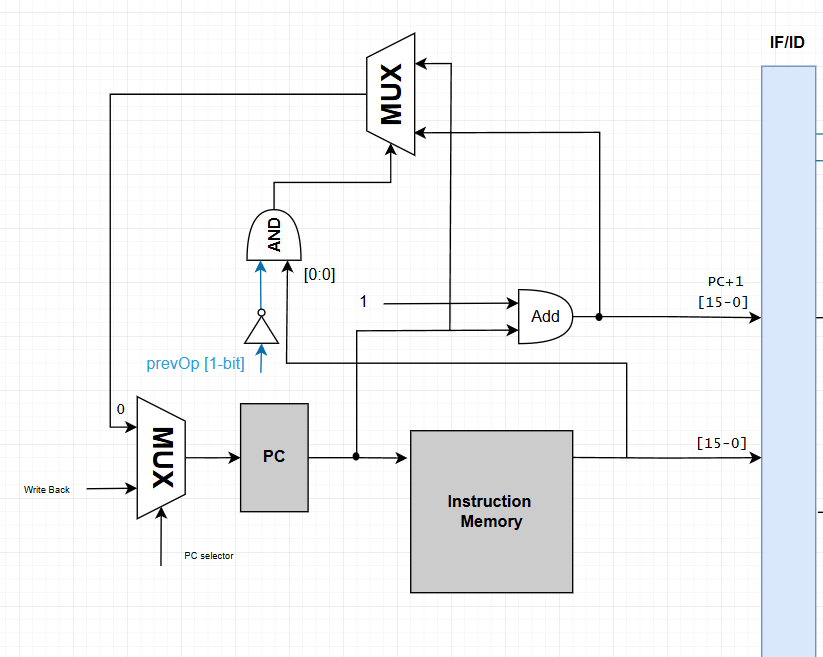
\includegraphics[width=\textwidth]{./assets/IF.png}
\end{center}
\end{minipage}


\subsection*{ID (Instruction Decode)}
\begin{minipage}{0.6\textwidth}
\begin{itemize}
    \item Decode the instruction opcode and extract the necessary fields.
    \item Read the register file to get the values of the source registers.
    \item Determine the type of instruction and the required control signals.
    \item Calculate the effective address for memory operations if applicable.
    \item Forward register values and immediate operands to the next stage (EX).
    \item Stall the pipeline if a data hazard is detected and cannot be resolved with forwarding.
\end{itemize}
\end{minipage}
\begin{minipage}{0.35\textwidth}
\begin{center}
    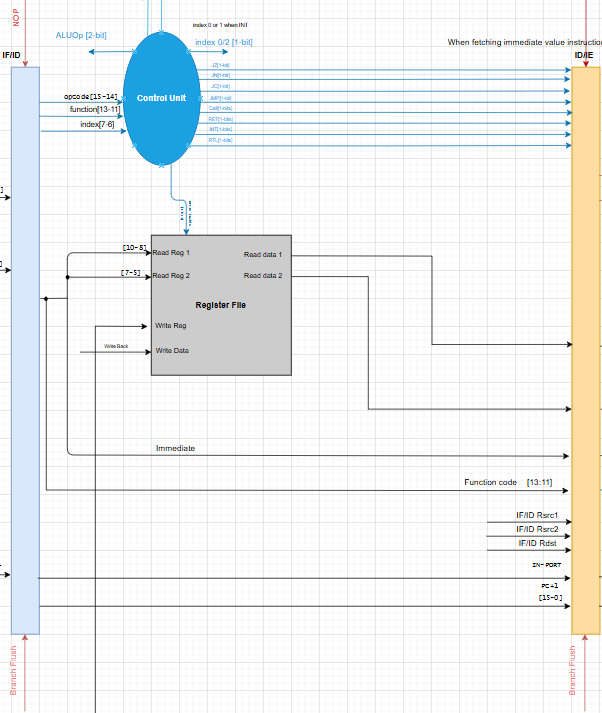
\includegraphics[width=\textwidth]{./assets/ID.png}
\end{center}
\end{minipage}

\subsection*{EX (Execution Stage)}
\begin{minipage}{0.6\textwidth}
\begin{itemize}
    \item Select ALU inputs through multiplexers based on control signals (\texttt{ALUsrc1} and \texttt{ALUsrc2}).
    \item Perform the ALU operation based on the control signals (\texttt{ALUOp}) and the instruction’s function field (\texttt{Func[3-bit]}).
    \item Generate the condition flags (\texttt{ZF, NF, CF}) based on the ALU result.
    \item Calculate the branch target address if the instruction is a branch or jump.
    \item Evaluate the branch condition using flags and control signals (\texttt{JMP}, \texttt{CALL}, \texttt{JC}, \texttt{JZ}, \texttt{JN}).
    \item Forward the ALU result to the Memory Access (MEM) stage.
    \item Stall the pipeline if a data hazard is detected and cannot be resolved with data forwarding.
    \item Flush the pipeline if a branch instruction is mispredicted.
    \item Generate control signals to update the Program Counter (PC) if a branch is taken.
\end{itemize}
\end{minipage}
\begin{minipage}{0.35\textwidth}
\begin{center}
    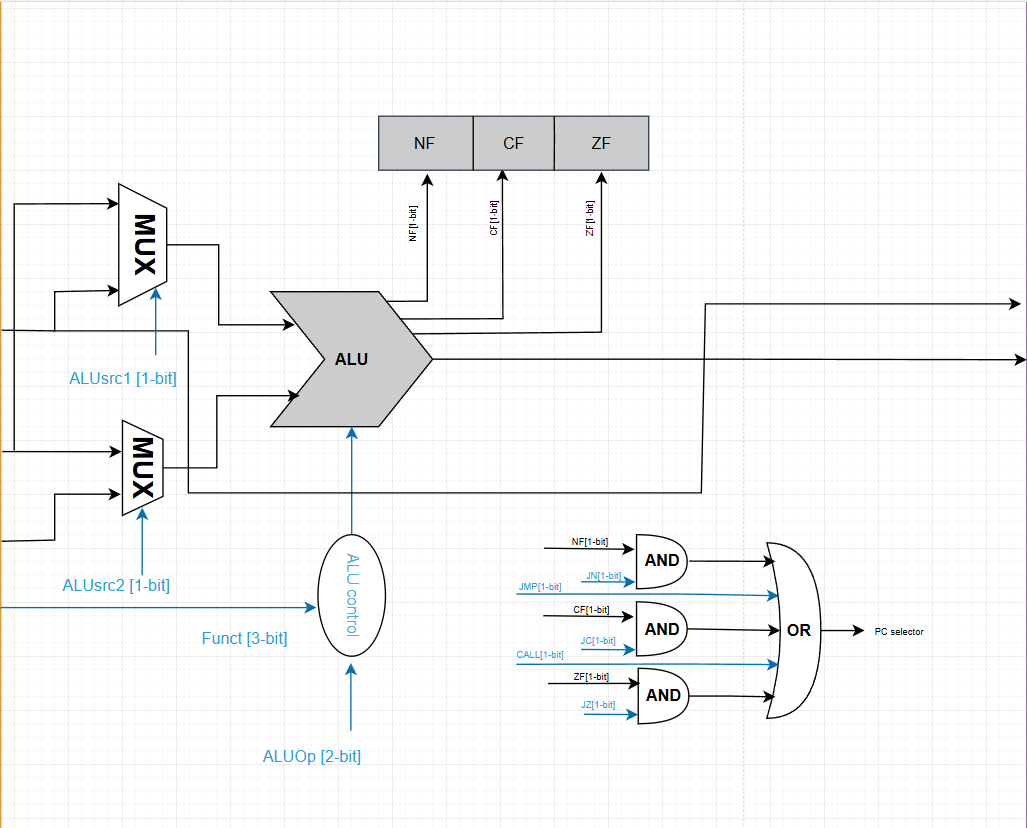
\includegraphics[width=\textwidth]{./assets/EX.png}
\end{center}
\end{minipage}

\subsection*{MEM (Memory Access)}
\begin{minipage}{0.6\textwidth}
\begin{itemize}
    \item Access memory to read or write data based on the instruction type.
    \item Forward the memory read data to the Write Back (WB) stage.
    \item Stall the pipeline if a data hazard is detected and cannot be resolved with data forwarding.
    \item Stack control unit handles stack operations (PUSH, POP).
    \item Control unit generates signals to enable memory read/write operations.
    \item If the instruction doesn't involve memory access, forward the ALU result to the WB stage.
\end{itemize}
\end{minipage}
\begin{minipage}{0.35\textwidth}
\begin{center}
    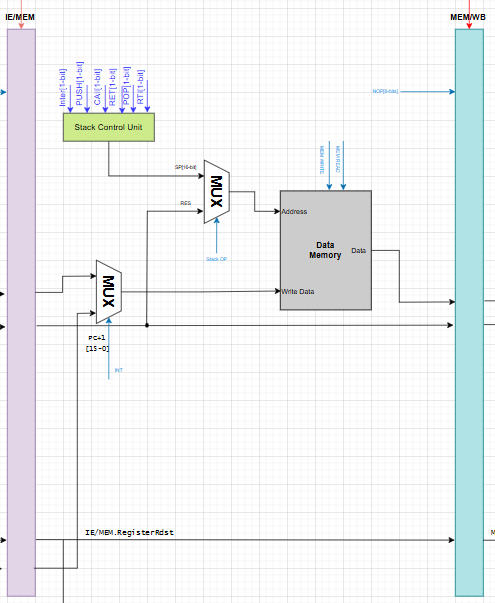
\includegraphics[width=\textwidth]{./assets/MEM.png}
\end{center}
\end{minipage}

\subsection*{WB (Write Back)}
\begin{minipage}{0.6\textwidth}
\begin{itemize}
    \item Update the register file with the new value if the instruction is a register operation.
    \item Update the Program Counter (PC) with the branch target address if a branch is taken.
    \item Stall the pipeline if a data hazard is detected and cannot be resolved with data forwarding.
    \item If the instruction is a jump or call, update the PC with the target address.
    \item If the instruction is a return, update the PC with the return address.
    \item If the instruction is a halt, stop the processor.
\end{itemize}
\end{minipage}
\begin{minipage}{0.35\textwidth}
\begin{center}
    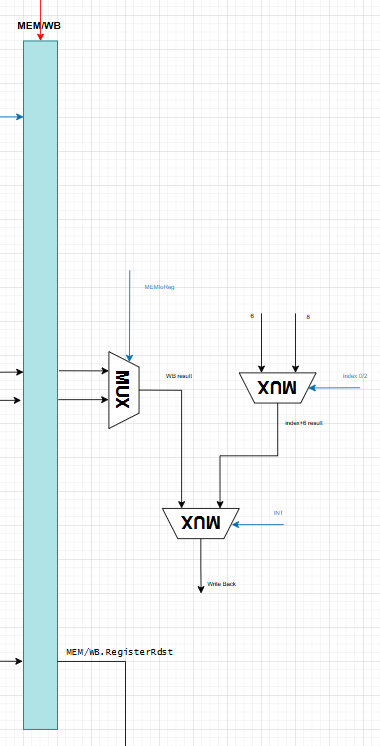
\includegraphics[width=\textwidth]{./assets/WB.png}
\end{center}
\end{minipage}


\section*{Conclusion}
This ISA defines a compact instruction encoding scheme with distinct categories to handle arithmetic, memory, and control operations efficiently. The use of 2-bit opcodes and 3-bit function fields allows for flexible expansion while maintaining a clear structure for decoding.

\end{document}
